%%%%%%%%%%%%%%%%%%%%%%%%%%%%%%%%%%%%%%%%%%%%%%%%%%%%%%%%%%%%%%%%%%%%%%
% How to use Overleaf: 
%
% You edit the source code here on the left, and the preview on the
% right shows you the result within a few seconds.
%
% Bookmark this page and share the URL with your co-authors. They can
% edit at the same time!
%
% You can upload figures, bibliographies, custom classes and
% styles using the files menu.
%
%%%%%%%%%%%%%%%%%%%%%%%%%%%%%%%%%%%%%%%%%%%%%%%%%%%%%%%%%%%%%%%%%%%%%%

\documentclass[12pt]{article}

\usepackage{sicti-template}

\usepackage{graphicx}

\usepackage[brazil]{babel}   

% FOR THOSE PAPERS WRITTEN IN ENGLISH
 % \addto\captionsbrazil{%
 % \renewcommand\refname{References}
 % \renewcommand{\figurename}{Figure}
 % \renewcommand{\tablename}{Table}
 % \renewcommand{\listfigurename}{List of Figures} 
 % \renewcommand{\listtablename}{List of Tables}
 % \renewcommand{\contentsname}{Contents}
 % \renewcommand\chaptername{Chapter}
 % }


\usepackage[utf8]{inputenc}
\usepackage{hyperref}

\usepackage[alf]{abntex2cite}	% Citações padrão ABNT

\usepackage{fancyhdr}
\pagestyle{fancy}

\fancyhead[L]{ }
\fancyhead[R]{ }

\chead{\begin{picture}(3,3) \put(-230,-15) {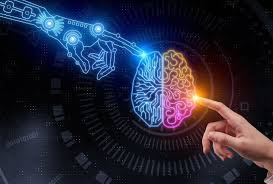
\includegraphics[width=16cm, height=2.8cm, keepaspectratio=false]{descarga (3).jpeg}} \end{picture}}
\renewcommand{\headrulewidth}{0pt}
\sloppy



\begin{document} 



\title{\begin{picture}(3,3) \put(-70,30){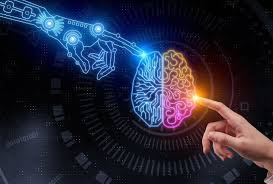
\includegraphics[width=16cm, height=2.8cm, keepaspectratio=false]{descarga (3).jpeg}} \end{picture}
La inteligencia artificial generativa y su impacto en la creación
de contenidos mediáticos}

\author{Chica Gomez Ruth Estefania\inst{1}}
  


\address{ Tecnologias de la informacion y comunicacion (TIC) \\ Universidad Laica Eloy de Manabí(ULEAM)\\
  El Carmen Manabí
\nextinstitute
  Etudiante de ingeniería en Tecnologias de la informacion \\ Inteligencia artificial
  \\
  Catedrático: Ing. César Sinchiguano 
  \email{\{8 vo \}Semestre}
}

\maketitle

\begin{abstract}
  The study examines the advantages, disadvantages and dangers of generative artificial intelligence (AI) for media content creation, including language models, adversarial networks, deepfake technology, and how it affects intellectual property, culture and lives.\\
  \textbf{Keywords:} creative algorithms, media content, ethics of technology, artificial intelligence, generative models
\end{abstract}
     
\begin{resumo} 
El estudio examina las ventajas, desventajas y peligros de la inteligencia artificial (IA) generativa para la creación de contenido en los medios, incluidos modelos de lenguaje, redes antagónicas, tecnología deepfake, y cómo afecta la propiedad intelectual, la cultura y la vida.\\
  \textbf{Palabras clave:} algoritmos creativos, contenidos mediáticos, ética de la tecnología, inteligencia artificial, modelos generativos

\end{resumo}


\section{Introducción}
El objetivo de la disciplina científica y tecnológica de la inteligencia artificial (AI) es crear sistemas capaces de resolver tareas que normalmente requieren la inteligencia humana. Gracias a tres factores: algoritmos sofisticados, mayor capacidad de cálculo y acceso a grandes cantidades de datos, ha hecho un gran avance. La inteligencia artificial tiene aplicaciones en una variedad de campos, como medicina, finanzas, meteorología y transporte. Las inteligencias artificiales son simbólicas, basadas en datos y basadas en contexto. El primero es responsable del crecimiento actual de la IA, mientras que el segundo es incierto y complejo, con el objetivo de comprender el mundo real y ofrecer soluciones innovadoras a problemas nuevos o desconocidos. La inteligencia artificial se ha utilizado principalmente para crear contenido automatizado, utilizando redes neurales y procesos de aprendizaje automático.\\
La IA generativa ha aumentado su capacidad tecnológica y es avanzando en la creatividad humana. Sin embargo, la seguridad de la herramienta depende del uso que se le desempeña. La IA puede provocar nuevos problemas si no se usa apropiadamente. En últimos años, iniciativas sociales como OpenAI, OdiseIA y Google's AI for Social Good programa promueven el uso ético y responsable de la IA. Se espera que el impacto de La IA en el trabajo, la economía y la educación sea significativo para 2030. En los medios de comunicación, la IA puede facilitar el trabajo de profesionales, pero también entrar riesgos para la originalidad, calidad y veracidad de los contenidos.
% Conferences that publish just abstracts ask for \textbf{one}-page texts.

\section{ Metodología} \label{sec:firstpage}
La revisión bibliográfica se a basado en búsquedas sistemáticas en bases de datos como Scopus, Web of Science, Google Académico, Bing y Google, utilizando términos representativos para la investigación. Los resultados más relevantes se filtran utilizando criterios como la fecha de publicación, la lengua, el tipo de documentos y la relevancia del tema. Un resumen completo identificando tendencias, controversias y desafíos en la utilización de la inteligencia generativa en la comunicación desde una perspectiva ética y legal.
\\Los modelos de IA se entrenan con grandes conjuntos de datos para aprender patrones y reglas. Los modelos de IA pueden generar contenido nuevo basado en el aprendizaje realizado.El contenido generado por IA se evalúa y refina para mejorar su calidad y precisión.

% \section{CD-ROMs and Printed Proceedings}

%In some conferences, the papers are published on CD-ROM while only the
%abstract is published in the printed Proceedings. In this case, authors are
%invited to prepare two final versions of the paper. One, complete, to be
%published on the CD and the other, containing only the first page, with
%abstract and ``resumo'' (for papers in Portuguese).

\section{ Un nuevo paradigma en la creación de contenidos}

La IA generativa es una herramienta valiosa para la producción de contenido en los medios de comunicación, especialmente en periodismo, creación gráfica, audiovisual y entretenimiento. Estos avances generan textos, voces y imágenes automatizadas, simplificando tareas y reduciendo tiempos de producción. Sin embargo, resuelve importantes éticos, como transparencia, responsabilidad, riesgo de contenidos, protección de privacidad y autorechos. A continiacion algunos aspectos:
\begin{itemize}
    \item Automatización de tareas: La IA puede automatizar tareas repetitivas como la redacción de noticias o la creación de imágenes simples.
    \item Creatividad y originalidad: Los modelos de IA pueden generar contenido original y creativo que va más allá de la capacidad humana.
    \item Personalización y segmentación:La IA puede personalizar el contenido para diferentes audiencias y plataformas.
    \item Acceso a nuevas formas de expresión:La IA abre nuevas posibilidades para la creación de contenido con diferentes formatos y estilos
\end{itemize}
\subsection{Redacción automatizada de noticias}

El GPT, el modelo Generative Pre-trained Transformer, diseñado por OpenAI para producer textos con el estilo, tono y arquitectura de la escritura humana, es una aplicación del aprendizaje profundo que ha difícil distinguir de los redactados por una persona.
\\Ventajas
\begin{itemize}
    \item Mayor rapidez y eficiencia en la producción de noticias.
    \item Posibilidad de generar contenido personalizado.
    \item Acceso a información y datos en tiempo real.
\end{itemize}


\subsection{ Síntesis de imágenes a partir de texto}\label{sec:figs}
Gracias a herramientas como Craigon, DALL·E, Midjourney y Stable Diffusion, la creación de imágenes basadas en texto se popularizó en 2022. Utilizando breves inputs de lengua natural, estas aplicaciones pueden generar imágenes originales de una variedad de tipos, como objetos, animales, paisajes y personas. Los conjuntos de generación basados en el aprendizaje profundo, que utilizan el aprendizaje profundo para instruir grandes cantidades de datos, pueden generar imágenes impresionantes, pero también pueden presentar problemas y peligros. \\Los modelos genéticos pueden reproducir la segregación racial, cultural y de género, lo que requiere algorithmos para corregir las desviaciones para la equidad. Falsas imágenes también pueden debilitar la confiabilidad de la prueba visual, lo que conduce a información errónea. 
Si bien la IA generativa puede tener importancia histórica, también puede producir ilustraciones abstractas y conceptuales, que podrían tener un impacto en los profesionales de la fotografía y la ilustración.
\begin{figure}
    \centering
    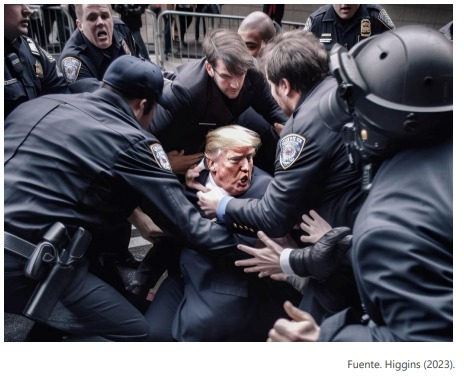
\includegraphics[width=0.5\linewidth]{WhatsApp Image 2024-09-18 at 20.52.39.jpeg}
    \caption{Falsas imágenes de Donald Trump arrestado por la policía, generadas con Midjourney}
    \label{fig:enter-label}
\end{figure}


\subsection{Vídeos hipertrucados: tecnología deepfake}

La manipulación de videos es casi tan antigua como el contenido audiovisual en sí. Desde sus inicios, se han utilizado técnicas para modificar videos, como recortarlos o editarlos , con el fin de cambiar su contexto, agregar elementos nuevos o, por ejemplo, simular el estado de ebriedad de quienes aparecen en ellos. Aunque estos métodos alteran el material original, no alteran la apariencia o las declaraciones de los personajes principales. Sin embargo, la tecnología deepfake es una nueva forma de producir contenido falso que presenta un desafío moral y social en los últimos años. Esta tecnología utiliza la IA generativa para producir videos con un nivel de realismo tan alto que es difícil determinar si son falsos. A diferencia de métodos previos, los videos deepfake.
\begin{itemize}
    \item La IA puede crear vídeos hiperrealistas que manipulan la apariencia de las personas.
    \item Efectos especiales en películas y series.
    \item Creación de contenido educativo y de entretenimiento.
    \item Posibilidad de uso indebido para crear desinformación y propaganda.
    \item Amenaza a la privacidad y a la seguridad de las personas.
\end{itemize}

\subsection{Síntesis de vídeo a partir de texto}\label{sec:figs}

Además, los modelos generativos permiten crear videos sintéticos a partir de indicaciones de texto simples.
Aunque es una tecnología que se basa en la síntesis de imágenes, los desarrollos como Make-A-Video de Meta, NUWA-XL de Microsoft y Phenaki de Google muestran un gran potencial creativo.
Estas herramientas permiten crear secuencias de video en minutos sin necesidad de material audiovisual previo, lo que puede ser una herramienta útil para los artistas. Solo se necesita proporcionar una base de texto para trabajar y el software crea un video listo para usar.\\
La síntesis de vídeo con IA generativa no es original o innovada, es limitada a reproducir estilos visuales de épocas anteriores de cine y televisión, conformando a la imitación de culturales precedentes como forma de consumo digital. La falta de originalidad también afecta a las plataformas de streaming desde hace tiempo.
\begin{itemize}
    \item Creación de contenido visual dinámico.
    \item Acceso a nuevas formas de narrar historias.
    \item Posibilidad de generar contenido personalizado.
\end{itemize}

\subsection{Clonación de voz}
La síntesis del habla es una tecnología sencilla que convertir texto en una voz parecida a la humana. Esta tecnología se utiliza en situaciones diversas, como voz assistantes, lectores de pantalla, navegación GPS, idiomas aprendizaje y atención telefónica automatizada. A pesar de avances en aprendizaje profundo, las posibilidades comerciales de la síntesis de voz han ampliado. Una fórmula pionera es la clonación de voces famosas para usarlas en audiolibros, productos audiovisuales y entornos inmersivos. La IA es una ventaja para tareas expertas sin coste o trabas que supone contratar a una persona experta. Sin embargo, el sector del doblaje se teme ante las prometedoras posibilidades de la síntesis de voz. Los medios de comunicación pueden usar voces clonadas para otros fines, como narrar noticias y eventos, o dar voz a personajes históricos o fallecidos en documentales y programas de televisión.
\begin{itemize}
    \item La IA puede generar audio con la voz de una persona específica.
    \item Creación de audiolibros y podcasts.
    \item Doblaje de películas y series.Generación de contenido interactivo.
    \item Riesgos: Posibilidad de uso indebido para el fraude y la suplantación de identidad.
    \item Amenaza a la seguridad y la privacidad de las personas.
\end{itemize}

\begin{figure}
    \centering
    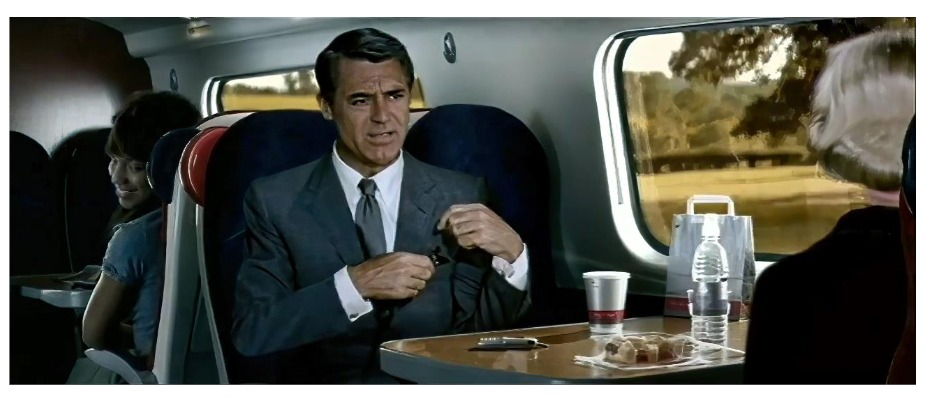
\includegraphics[width=0.5\linewidth]{WhatsApp Image 2024-09-18 at 20.47.33.jpeg}
    \caption{Protagonistas de Con la muerte en los talones (1959) insertados en un tren de Virgin Trains
(2005), ante la sorpresa de una usuaria moderna.}
    \label{fig:enter-label}
\end{figure}

\section{ Discusión y conclusiones}
La IA generativa es una tecnología clave para el periodismo y los medios de comunicación, y es de creciente relevancia en la producción de contenidos. Algoritmos generan contenido nuevo a través de indicaciones sencillas, simples descripciones o parámetros básicos. Sin embargo, se ayuda a una adopción generalizada de estos sistemas, lo que proporciona que el contenido automático sea cada vez más habitual y ubicuo. Sin embargo, se deben aumentar la conciencia pública sobre el uso responsable y ético de esta tecnología.
\subsection{Hacia una ética de la IA y Futuras líneas de investigación}
Es crucial desarrollar una ética de la IA para garantizar un uso responsable y transparente de esta tecnología. Las futuras líneas de investigación se centrarán en mejorar la calidad y la seguridad del contenido generado por IA, así como en abordar las implicaciones éticas y sociales de esta tecnología en constante evolución.\\

\section{Bibliografía}
Franganillo, J. (2023). La inteligencia artificial generativa y su impacto en la creación de contenidos mediáticos. Methaodos Revista De Ciencias Sociales, 11(2), m231102a10. https://doi.org/10.17502/mrcs.v11i2.710\\
Ajder, H. (2020). Deepfake threat intelligence: a statistics snapshot from June 2020. Sensity.
Ajder, H., Patrini, G., Cavalli, F.,  Cullen, L. (2019). The state of deepfakes: landscape, threats, and impact.
DeepTrace. https://is.gd/LK0X5N\\
Ayuso, S., y Pascual, M. G. (2023, 11 de mayo). Europa quiere poner más obligaciones a la inteligencia artificial
generativa como la de ChatGPT. El País. https://is.gd/lQNRia\\
Barandy, K. (2022, 10 de agosto). Will artists be replaced by artificial intelligence? Designboom. https://is.gd/NZqVHX
Bender, E. M. (2022, 14 de junio). Human-like programs abuse our empathy: even Google engineers aren’t
immune. The Guardian. https://is.gd/rAUdbF\\
Bhargava, C., y Sharma, P.K. (Eds.) (2022). Artificial intelligence: fundamentals and applications. CRC Press.
Boden, M. A. (2018). Artificial intelligence: a very short introduction. Oxford University Press.\\
Botha, J., y Pieterse, H. (2020). Fake news and deepfakes: a dangerous threat for 21st century information
security. 15th International Conference on Cyber Warfare and Security: ICCWS 2020, 57-66.\\
Boucher, P. (2020). Artificial intelligence: how does it work, why does it matter, and what can we do about it?
Servicio de Estudios del Parlamento Europeo. https://doi.org/10.2861/44572\\
Broderick, R. (2023, 31 de mayo). AI can’t replace humans yet: but if the WGA writers don’t win, it might not
matter. Polygon. https://is.gd/PT9hSr\\
Campesato, O. (2020). Artificial intelligence, machine learning and deep learning. Mercury Learning and
Information.\\
Castillo, C. (2023, 3 de mayo). Los creadores del canon AEDE quieren una “tasa ChatGPT” para la inteligencia
artificial. elDiario.es. https://eldiario.es/1-9b351c\\
Dean, I. (2022, 11 de agosto). You can now sell your DALL·E 2 art, but it feels murky. Creative bloq. https://is.gd/ov3In5\\
Dale, R. (2022). The voice synthesis business: 2022 update. Natural language engineering, 28(3), 40-408.
https://doi.org/10.1017/S1351324922000146\\
Davenport, T. H., y Mittal, N. (2022, 14 de noviembre). How generative AI is changing creative work. Harvard
Business Review. https://is.gd/by7hQt\\
Giannini, S. (2023). Generative AI and the future of education. UNESCO. https://is.gd/CbhGO5\\
Giansiracusa, N. (2021). How algorithms create and prevent fake news: exploring the impacts of social media,
deepfakes, GPT-3 and more. Apress. https://doi.org/10.1007/978-1-4842-7155-1\\
Greenhouse, (2023, 8 de febrero). US experts warn AI likely to kill off jobs and widen wealth inequality. The
Guardian. https://is.gd/n38xQn\\
Hao, K. (2021, 3 de febrero). Internet está tan sesgado que, para la IA, las mujeres solo llevan bikini. MIT
Technology Review. https://is.gd/kSOd56\\
Hatzius, J., Briggs, J., Kodnani, D., y Pierdomenico, G. (2023, 26 de marzo). The potentially large effects of
artificial intelligence on economic growth. Goldman Sachs.

\end{document}
